% !TEX root = ../../../report.tex

\FloatBarrier
\subsection{Communication Between the MCU and the \textit{ChaosM}}\label{section:fpga-buses}

\textit{ChaosM} on the FPGA communicates with the microcontroller using the external bus interface
(EBI) of the Giant Gecko microcontroller. Inside \textit{ChaosM}, an EBI controller is responsible
for servicing requests from the microcontroller and driving the internal bus, which
is used for transferring data to and from modules in the FPGA.

\subsubsection{The EBI Bus}
The EBI\cite{efm_ebi} is a parallel bus with a separate data and address bus, in
addition to chip select, read-enable, and write-enable signals.

The communication between the MCU and the FPGA uses 23 address lines and 16 data
lines. All transfers are initiated when the chip select signal goes low. For
write transfers, the data and address lines are set up and the write enable
signal is asserted, see figure \ref{fig:ebi_write}.

For reads, the address is set up and the data lines are put in high impedance mode
before the read enable signal is asserted, see figure \ref{fig:ebi_read}.

\begin{figure}[h]
	\centering
	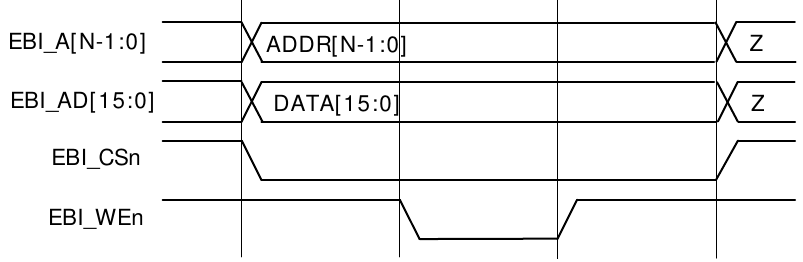
\includegraphics[width=0.8\linewidth]{figures/fpga/ebi_write.png}
	\caption{EBI write transfer\cite[p.6]{efm_ebi}}
	\label{fig:ebi_write}
\end{figure}



\begin{figure}[h]
	\centering
	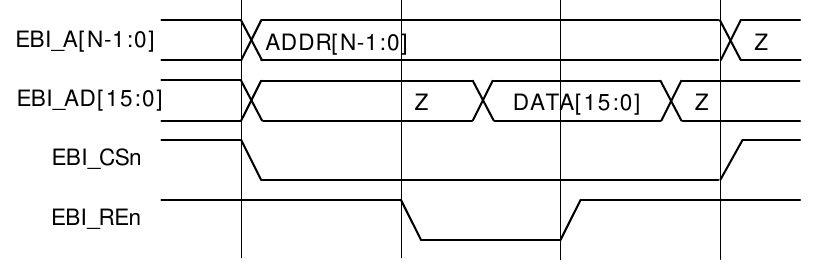
\includegraphics[width=0.8\linewidth]{figures/fpga/ebi_read.png}
	\caption{EBI read transfer\cite[p.7]{efm_ebi}}
	\label{fig:ebi_read}
\end{figure}



All data transfers are initiated by the microcontroller, which works as bus
master for the EBI bus. The EBI controller facilitates communication between
the EBI bus and the internal bus.

\FloatBarrier
\paragraph{Addressing}

The input/output, control registers, and pipelines in the FPGA are addressed
using a simple addressing scheme, where the address is divided into several
parts, as illustrated in figure \ref{fig:ebi_addresses}.

\begin{figure}[H]
	\centering
	\begin{bytefield}[endianness=big,bitwidth=0.04\linewidth]{23}
		\bitheader{0-22}\\
		\bitbox{1}{T} &
		\bitbox{2}{\tiny Pipeline} &
		\bitbox{4}{Device} &
		\bitbox{2}{\tiny Subdev} &
		\bitbox{14}{Address}
	\end{bytefield}
	\caption{FPGA address format}
	\label{fig:ebi_addresses}
\end{figure}




In an EBI address, the T bit is used to select the toplevel control register.
If the T bit is set, the rest of the address is ignored, and only the toplevel
control register is accessible. If the T bit is not set, the pipeline field is
used to select which pipeline to address. In a pipeline, the device
and subdevice fields are used to select which module in the pipeline to address.

Using this addressing scheme, the memory map, as seen from the MCU, becomes
like illustrated in figure \ref{fig:fpga_memmap}

\begin{figure}
	\begin{bytefield}[bitwidth=0.035\linewidth,rightcurly=.,rightcurlyspace=0pt,endianness=big]{23}
		\bitheader{0-22}\\
		\begin{rightwordgroup}{0x400000}
			\bitbox{23}{\textbf{Toplevel control register}}
		\end{rightwordgroup}\\
		\begin{rightwordgroup}{...}
			\bitbox{23}{(\textit{The rest of the cores in Pipeline 1})}
		\end{rightwordgroup}\\
		\begin{rightwordgroup}{0x144000}
			\bitbox{23}{Pipeline 1 - Core 0 instruction memory}
		\end{rightwordgroup}\\
		\begin{rightwordgroup}{0x140000}
			\bitbox{23}{Pipeline 1 - Core 0 control register}
		\end{rightwordgroup}\\
		\begin{rightwordgroup}{0x130000}
			\bitbox{23}{Pipeline 1 Output buffer}
		\end{rightwordgroup}\\
		\begin{rightwordgroup}{0x120000}
			\bitbox{23}{Pipeline 1 Input buffer}
		\end{rightwordgroup}\\
		\begin{rightwordgroup}{0x100000}
			\bitbox[blr]{23}{\textbf{Pipeline 1 control register}}
		\end{rightwordgroup}\\
		\begin{rightwordgroup}{...}
			\bitbox{23}{(\textit{The rest of the cores in Pipeline 0})}
		\end{rightwordgroup}\\
		\begin{rightwordgroup}{0x54000}
			\bitbox{23}{Pipeline 0 - Core 1 instruction memory}
		\end{rightwordgroup}\\
		\begin{rightwordgroup}{0x50000}
			\bitbox{23}{Pipeline 0 Core 1 control register}
		\end{rightwordgroup}\\
		\begin{rightwordgroup}{0x44000}
			\bitbox{23}{Pipeline 0 - Core 0 instruction memory}
		\end{rightwordgroup}\\
		\begin{rightwordgroup}{0x40000}
			\bitbox{23}{Pipeline 0 - Core 0 control register}
		\end{rightwordgroup}\\
		\begin{rightwordgroup}{0x30000}
			\bitbox{23}{Pipeline 0 Output buffer}
		\end{rightwordgroup}\\
		\begin{rightwordgroup}{0x20000}
			\bitbox{23}{Pipeline 0 Input buffer}
		\end{rightwordgroup}\\
		\begin{rightwordgroup}{0x00000}
			\bitbox{23}{\textbf{Pipeline 0 control register}}
		\end{rightwordgroup}\\
	\end{bytefield}

	\caption{FPGA memory map overview}
	\label{fig:fpga_memmap}
\end{figure}
\FloatBarrier
